\documentclass[index]{subfiles}

\begin{document}
\title{Ventilatory System Experiment}
\author{by Andy Li}
\date{26 November 2021}
\maketitle

\section{The meaning of the terms \textit{pulmonary ventilation}, \textit{total lung capacity}, \textit{vital capacity}, \textit{tidal volume}, \textit{expiratory reserve volume}, \textit{inspiratory reserve volume}, and \textit{residual volume}}

The ventilatory system is in charge of \textbf{pulmonary ventilation} (a fancy word for breathing), defined as the passing of air in and out of the lungs. There are several complex terms used to describe both the movement of air in and out of the lungs, as well as the volume of air itself.

These are better explained with a picture below.

\begin{figure}[H]
    \centering
    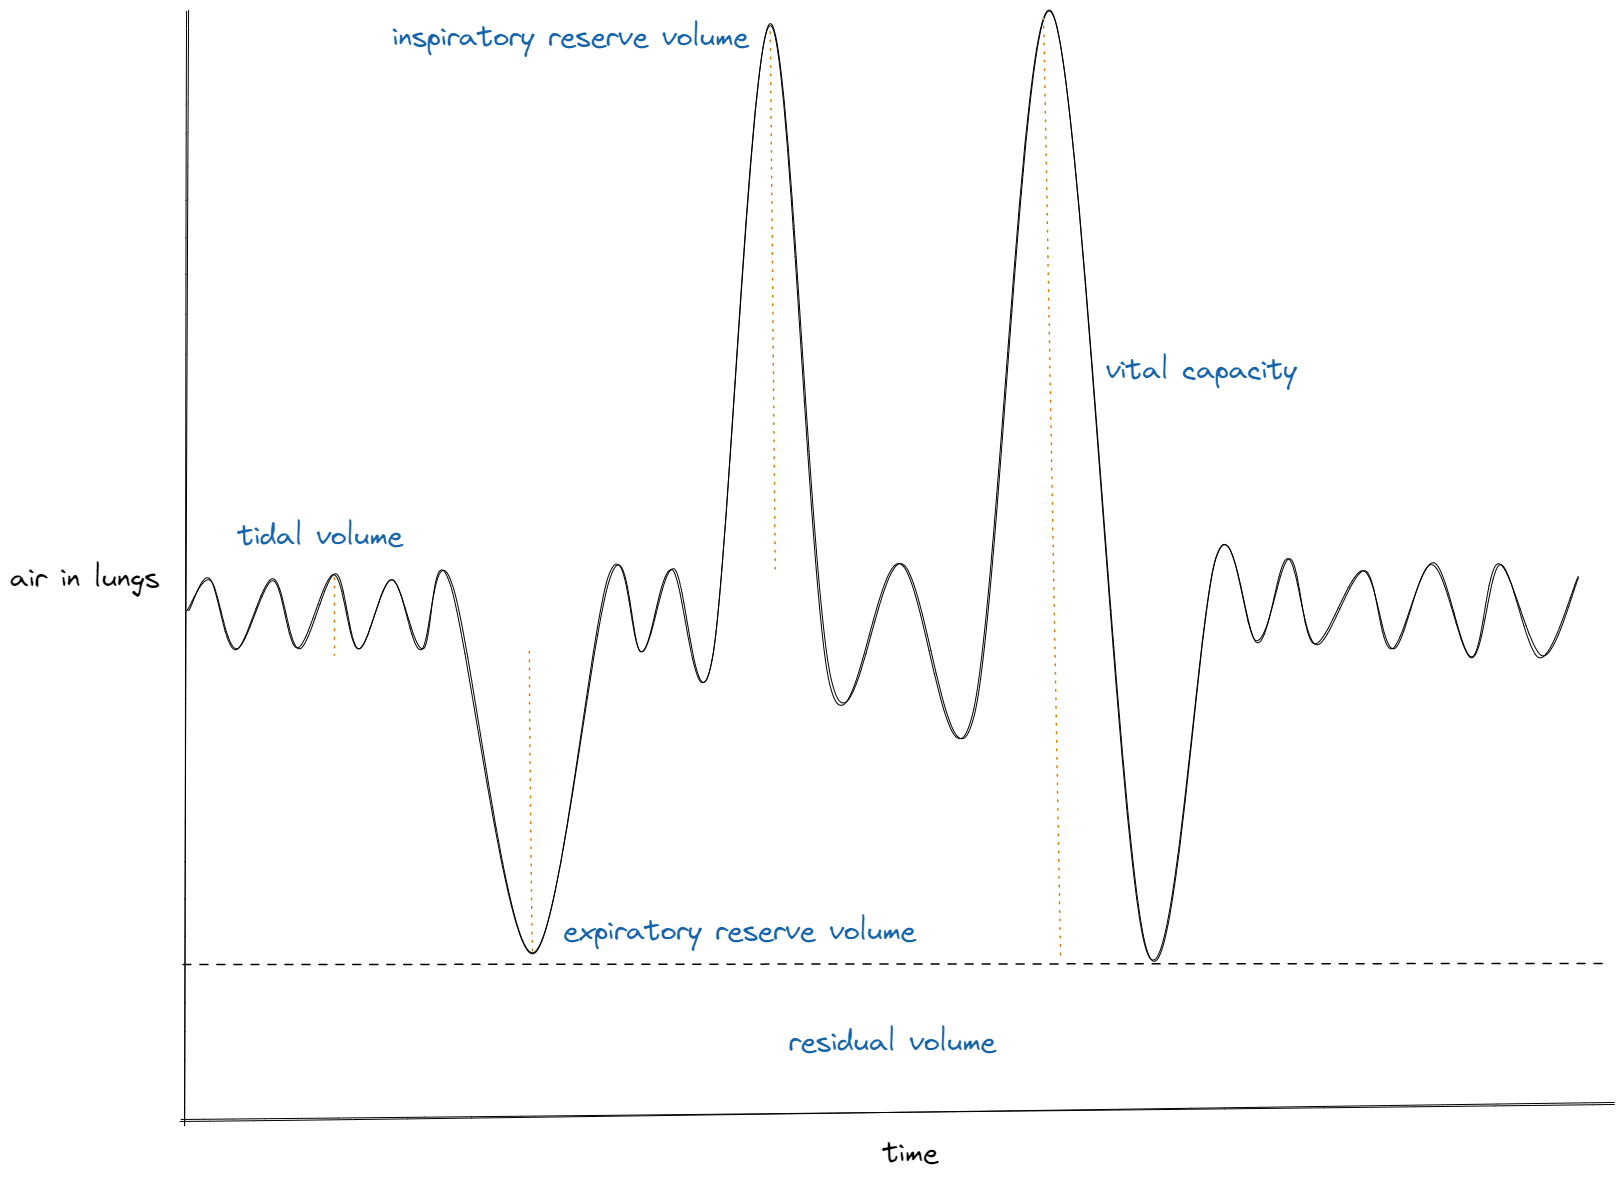
\includegraphics[scale=0.24]{respiratory_cycle.png}
    \caption{Graph of air volume in lungs after varying amounts of inspiration and expiration}
\end{figure}

First, understand that a \textbf{respiratory cycle} is an inspiration and expiration, or in other words, a breath in followed by a breath out. On the graph, this is could be thought of as going from one trough (low point) to another trough, or one crest (high point) to another crest.

Normal respiratory breathing is quiet, and isn't voluntary. In quiet breathing, the amount of air that enters during one inspiration, or the amount of air that exits during one expiration, is known as the \textbf{tidal volume}. On the graph, the fairly consistent small ups and downs at the beginning are indicative of quiet breathing, and their \(amplitude\times 2\) show tidal volume.

Of course, we can voluntarily take control of our respiratory muscles, and forcefully breathe in more air or expel more air than is normal during quiet breathing. When we take in as much air as possible, the extra amount of air moved into the lungs compared to a quiet inspiration is known as the \textbf{inspiratory reserve volume}.

On the graph, the second vertical dotted horizontal line that follows the high arc is representative of this inspiratory reserve volume.

The opposite of inspiratory reserve volume is \textbf{expiratory reserve volume}. We can force ourselves to breathe out as much air as possible, and the extra amount of air moved out of the lungs compared to a quiet expiration is konwn as the expiratory reserve volume.

However, compared to inspiratory reserve volume where we can fill up our lungs to the fullest, we can't actually expel out all the air in our lungs. The extra amount of air that can't be expelled is known as the \textbf{residual volume}, and it's indicated by the level dotted line on the graph near the bottom.

A maximum breath out after a maximum breath in is known as the \textbf{vital capacity}. Another way to think about it is
\[
    vital\ capacity = tidal\ volume + inspiratory\ reserve\ volume +expiratory\ reserve\ volume
\]
We add in tidal volume, because inspiratory reserve volume and expiratory reserve volume is the amount of \textit{extra} air you can breathe in and out compared to quiet breathing.

With all these volumes defined, we can now say that \textbf{total lung capacity}, the total voluem of air the lungs can store,  is equal to
\[
    total\ lung\ capacity = vital\ capacity + residual\ volume
\]

\section{The mechanics of ventilation in human lungs}

In order to breathe in, the diaphragm moves down, and thoracic cage moves up and outwards. This causes the lungs to expand, thus increasing the volume of the lungs. Because \(d=\frac{m}{v}\) (density is equal to mass over volume), as the volume of the lungs expand, the \textbf{intra-alveolar-pressure} (pressure inside the lungs) decreases, becoming less than atmospheric pressure. This causes the atmosphere to push air into the lungs. Because this air pressure difference is the force that is actually pushing air into the lungs, breathing in is known as a \textbf{negative pressure} system.

Then to breathe out, the natural elasticity of the respiratory muscles will cause the diaphragm and thoracic cage to return to their original positions, forcing air out. Extra force can also be voluntarily added to the thoracic cage, to accelerate the flattening of the lungs.

\begin{figure}[H]
    \centering
    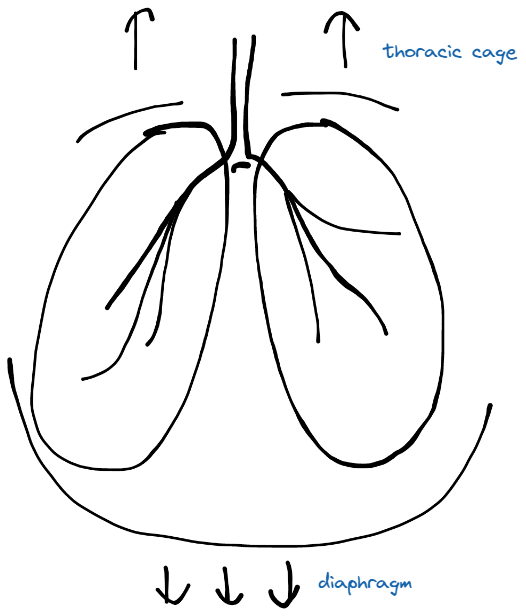
\includegraphics[scale=0.3]{lungs.png}
    \caption{Lungs in inspiration}
\end{figure}

\section{Research \& Writing}

\subsection{How do the lungs affect the performance of beginning and elite runners?}

Evidence shows that lungs generally do not affect the performance of runners in the way we think they do.

Most of the time, the lungs are already providing enough air for the body. According to Karp, total lung capacity doesn't have an effect on endurance running because oxygen is already near maximally saturated in hemoglobin. Hemoglobin is the protein responsible for carrying 98.5\% of the body's oxygen through the blood stream. It gets this oxygen through the elegant process of diffusion, a process where oxygen from the lungs moves into the blood stream due to a partial-pressure difference \citep{karp}. Evidence shows that even ``while running a race, this near-maximal saturation is maintained in healthy people.''

However, lungs may still impact performance in negative ways. Breathing too much may come at a cost to performance. According to Karp, during ``70\%'' maximal oxygen consumption, the ventilatory system makes up around ``3-6\%'' of the body's oxygen consumption, but during 100\% maximal oxygen consumptionl, the ventilatory system could use as much of ``10-15\%'' of the total body's oxygen, diverting needed oxygen away from leg muscles. When runners have special medical conditions, such as ``pulmonary pathology'' \citep{karp}, or when the altitude is very high, the lungs may have problems keeping up arterial oxygen saturation, and may limit performance. Or for elite athletes, as lungs do ``not adapt to training'', it may be a limiting factor on performance when all the other systems are trained to their genetic potential \citep{karp}.

\subsection{The effect that training has on lung adaptation and performance}

For most novice athletes, the limiting factors are not present in the venticular systems at all but the cardiovascular and metabolic systems \citep{karp}, which are in charge of moving blood to muscles, and accepting oxygen from blood. For elite athletes, as lungs do not adapt to training as much as other systems of the body do \citep{karp}, when the genetic potential of all other factors are reached, the lungs may ``lag'' behind the other systems and become a limiting factor. However, for novice runners, blaming their performance on the performance of their lungs is an unfounded argument.


\bibliography{citations.bib}

\end{document}
